% !TeX spellcheck = en_GB

\section{Algorithms}\label{algorithms}
\subsection{Sub modules}
Sub modules are parts of the algorithms that are denoted circled like \circled{A}, \circled{B}, \circled{C}, \circled{D} and \circled{E}. They are procedures that should to be explained in more detail a little bit for better understanding of the way of working of the algorithms.\\

\noindent \textbf{Distribute$(\Sigma,\ V) $ \circled{A} and Distribute$(V^2,\ V)$ \circled{B}:}\\
The difference between \circled{A} and \circled{B} is that one time $\Sigma$ and the other time $V^2$ are distributed. The specifics of how they are distributed are the same in both cases as described in the following algorithm: \\

\noindent
\frame{
	\begin{algorithm}[H] %or another one check
		\caption{Distribute}
		\label{Distribute}
		\SetAlgoLined
		\KwIn{ $Rhse \subseteq\ (V^{2} \cup \Sigma),\ V$}
		\KwOut{Set of productions $P \subseteq V \times (V^{2} \cup \Sigma)$}
		\ForEach{$rhse \in Rhse$}{
			$choose\ n\ uniform\ randomly\ in\ [i, j]$;~~\tcp{$i \in  \mathbb{N},\ j \in  \mathbb{N}$}
			$V_{add} := uniform\ random\ subset\ of\ size\ n\ from\ V$\; \label{sizeN}
			$P \cup \{ (v, rhse)\ |\ v \in V_{add},\ rhse \in Rhse \} $\;	
		}
		\Return $P$;
	\end{algorithm}
} \\

\noindent \textbf{Stopping Criteria \circled{C}:}\\
Two kinds of \circled{C} have been used. One is that it is true iff more than half of the pyramid cells are not empty and the other one is that there is at least one variable in the tip of the pyramid. It is to be taken in consideration that the latter is somewhat dependent on the count possible variables as seen in [XXX]. \\

\noindent \textbf{CalculateSubsetForCell(Pyramid, i, j) \circled{D}:}\\
This works kind of analogous from Line 7 to Line 9 of the CYK algorithm. For one $Cell_{i,j}$ every possible cell combination is looked at, i.e. if a rule like $lhse \rightarrow cs$ with $cs \in CellSet$ is added then automatically  $Cell_{i,j}$ won't be empty any more.\\

\noindent \textbf{Choose one xy with probability depending on row \circled{E} :}\\
There is the set $RowSet \subseteq \{(XY,i)\ |\ X,Y \in V \wedge i \in \mathbb{N} \}$\\
Compression of the RowSet like: (AB,3) and (AB,1) -> (AB,1) --> RowSetCompressed\\
rowListWeighted = add i times XY to rowListWeighted. XXX\\
\noindent Line \ref{rowSet}: $(AB,1), (AB,2), (BC,3) ... \in sub$ $\rightarrow$ multiple occurrences of $AB$ are allowed here yet.\\
$choose\ one~xy\ out\ of\ (XY,\ i) \in RowSet~uniform\ randomly\ with$ $probability~depending~on~i $\\

\noindent \frame{
	\begin{algorithm}[H] %or another one check
		\caption{CalculateSubsetForCell}
		\label{CalculateSubsetForCell}
		\SetAlgoLined
		\KwIn{$Pyramid,~i \in  \mathbb{N},\ j \in  \mathbb{N}$ }
		\KwOut{$CellSet \subseteq V^2$}
		$CellSet=\emptyset$\;
		\For{$k:=i-1 \to 0$}{ \label{cellCombs}
			$CellSet \cup \{X\ |\ X\longrightarrow YZ,\ Y \in Cell_{k,j},\ Z \in Cell_{i-k-1,k+j+1} \}$\;
		}
		\Return $CellSet$;

	\end{algorithm}
}
In the following situation a rule should be added so that $Cell_{3,0}$ won't be empty: 
\noindent
\begin{figure}[h]
	\begin{minipage}{6in}
		\centering
		\raisebox{-0.5\height}{
			\begin{tabular}{l}
				Grammar:\\
				$A \rightarrow AB~|~a$\\
				$B \rightarrow \textcolor{gray}{\textbf{SC}}~|~b$\\ 
				$C \rightarrow AB$ \\
				$S \rightarrow BA~|~AA$
			\end{tabular} 
		}
		\hspace*{.2in}
		\raisebox{-0.5\height}{
			\resizebox{0.5\linewidth}{!}{
				\resizebox{\linewidth}{!}{
					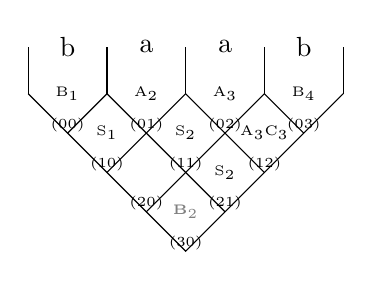
\begin{tikzpicture}[baseline]
					\newcommand{\myfontvars}[1]{
						\fontsize{4.9}{12}\selectfont{#1}
					}\newcommand{\myfontnumbering}[1]{
						\fontsize{2.5}{12}\selectfont{#1}
					}%Outer hull
					%Tip of the pyramid
					\coordinate (tip) at (2.0,-2.0);
					\foreach \i in {0,...,4} {
						\coordinate (\i) at (\i,0);
					}
					%Draw the left and right line of the pyramid pointing downwards
					\draw (0) -- (tip) -- (4);
					%Grid lines direction down-left to top-right
					\coordinate (dl1) at (0.5,-0.5);
					\coordinate (dl2) at (1.0,-1.0);
					\coordinate (dl3) at (1.5,-1.5);
					\draw (dl1) -- (1,0);
					\draw (dl2) -- (2,0);
					\draw (dl3) -- (3,0);
					%Grid lines direction down-right to top-left
					\coordinate (dr1) at (2.5,-1.5);
					\coordinate (dr2) at (3.0,-1.0);
					\coordinate (dr3) at (3.5,-0.5);
					\draw (dr1) -- (1,0);
					\draw (dr2) -- (2,0);
					\draw (dr3) -- (3,0);
					%Small lines at the top
					\coordinate (top0) at (0.0,0.0);
					\coordinate (top1) at (1.0,0.0);
					\coordinate (top2) at (2.0,0.0);
					\coordinate (top3) at (3.0,0.0);
					\coordinate (top4) at (4.0,0.0);
					\coordinate (topUpper0) at (0.0,0.6);
					\coordinate (topUpper1) at (1.0,0.6);
					\coordinate (topUpper2) at (2.0,0.6);
					\coordinate (topUpper3) at (3.0,0.6);
					\coordinate (topUpper4) at (4.0,0.6);
					\draw (top0) -- (topUpper0);
					\draw (top1) -- (topUpper1);
					\draw (top2) -- (topUpper2);
					\draw (top3) -- (topUpper3);
					\draw (top4) -- (topUpper4);
					%The string
					\coordinate (w0) at (0.5,0.6);
					\coordinate (w1) at (1.5,0.6);
					\coordinate (w2) at (2.5,0.6);
					\coordinate (w3) at (3.5,0.6);
					\node [] at (w0) {b};
					\node [] at (w1) {a};
					\node [] at (w2) {a};
					\node [] at (w3) {b};
					% Variables in the cells
					%cells00
					\coordinate (center00) at (0.5,0.0);
					\node [below=0.18cm] at (center00) {\myfontnumbering{$(00)$}};
					\node [] at (center00) {\myfontvars{B$_{1}$}};
					%cells01
					\coordinate (center01) at (1.5,0.0);
					\node [below=0.18cm] at (center01) {\myfontnumbering{$(01)$}};
					\node [] at (center01) {\myfontvars{A$_{2}$}};
					%cells02
					\coordinate (center02) at (2.5,0.0);
					\node [below=0.18cm] at (center02) {\myfontnumbering{$(02)$}};
					\node [] at (center02) {\myfontvars{A$_{3}$}};
					%cells03
					\coordinate (center03) at (3.5,0.0);
					\node [below=0.18cm] at (center03) {\myfontnumbering{$(03)$}};
					\node [] at (center03) {\myfontvars{B$_{4}$}};
					%cells10
					\coordinate (center10) at (1.0,-0.5);
					\node [below=0.18cm] at (center10) {\myfontnumbering{$(10)$}};
					\node [] at (center10) {\myfontvars{S$_{1}$}};
					%cells11
					\coordinate (center11) at (2.0,-0.5);
					\node [below=0.18cm] at (center11) {\myfontnumbering{$(11)$}};
					\node [] at (center11) {\myfontvars{S$_{2}$}};
					%cells12
					\coordinate (center12) at (3.0,-0.5);
					\node [below=0.18cm] at (center12) {\myfontnumbering{$(12)$}};
					\node [] at (center12) {\myfontvars{A$_{3}$C$_{3}$}};
					%cells20
					\coordinate (center20) at (1.5,-1.0);
					\node [below=0.18cm] at (center20) {\myfontnumbering{$(20)$}};
					%cells21
					\coordinate (center21) at (2.5,-1.0);
					\node [below=0.18cm] at (center21) {\myfontnumbering{$(21)$}};
					\node [] at (center21) {\myfontvars{S$_{2}$}};
					%cells30
					\coordinate (center30) at (2.0,-1.5);
					\node [below=0.18cm] at (center30) {\myfontnumbering{$(30)$}};
					\node [] at (center30) {\myfontvars{\textcolor{gray}{\textbf{B$_{2}$}}}};
					\end{tikzpicture}
				}	
			}
		}
	\end{minipage}
\end{figure}\\
Then the calculation of CellSet for $Cell_{3,0}$ results in $\{SA,~SC,~BS\}$, whereas $SA$ and $SC$ stem from $Cell_{1,0}$ together with $Cell_{1,2}$ and $BA$ is from $Cell_{0,0}$ together with $Cell_{2,1}$. Now if either one of the rules $lhse \rightarrow SA$, $lhse \rightarrow SC$ or  $lhse \rightarrow BS$ is added to the grammar, then $lhse\in Cell_{3,0}$. Here the rule  \textcolor{gray}{\textbf{B $\rightarrow$ SC}} has been added and now $B$ is element of $Cell_{3,0}$.

\subsection{DiceRollOnlyCYK}
\noindent This is a naive way of generating grammars, which will be the lower boundary while comparing the algorithms. Each future algorithm should have a higher score than this algorithm or otherwise it would be worse, than simple dice rolling the distribution of terminals (Line \ref{diceRollOnlyA}) and compound variables (Line \ref{diceRollOnlyB}). \\

\noindent
\frame{
	\begin{algorithm}[H] %or another one check
		\caption{DiceRollOnlyCYK}
		\label{DiceRollOnlyCYK}
		\SetAlgoLined
		\KwIn{Word $w \in \Sigma^{*}$ }
		\KwOut{Set of productions $P$}
		$P = \emptyset$;~~\tcp{$P \subseteq V \times (V^{2} \cup \Sigma)$}
		$P = Distribute(\Sigma,\ V)$;  \circled{A}\\ \label{diceRollOnlyA}
		$P \cup Distribute(V^2,\ V)$;  \circled{B}\\ \label{diceRollOnlyB}
		\Return $P$\;
	\end{algorithm}
}
A terminal $\Sigma$ is distributed to at least one $lhse$, but a compound variable $V^2$ must not be distributed at all. This means that for each terminal of $\Sigma=\{a,b\}$ there exists at least one rule like $lhse\rightarrow a$ and $lhse\rightarrow b$ and for each possible compound variable $V^2=\{AA,~AB,~AC,~AS,~BB,~BC,~BS,~CC,$ $~CS,SS\}$ it is possible that only a smaller subset like $\{AA,~BA,~CC,~SC\}$ is distributed so that only rules like $lhse\rightarrow AA$, $lhse\rightarrow BA$, $lhse\rightarrow CC$ and $lhse\rightarrow SC$ exist.
\noindent
\begin{figure} [h]
	\begin{minipage}{6in}
		\centering
		\raisebox{-0.5\height}{
			\begin{tabular}{l}
				Grammar after Line 2:\\
				$C\rightarrow a$\\ 
				$B\rightarrow b$\\
				\\
			\end{tabular} 
		\begin{tabular}{l}
			Grammar after Line 3:\\
			$C\rightarrow BA~|~AA~|~a$\\ 
			$B\rightarrow b$ \\
			$S\rightarrow CC~|~SC$ 
		\end{tabular}
	} 		
	\end{minipage}
	\caption{Short example of Algorithm \ref{DiceRollOnlyCYK}.}
	\label{DiceRollONlyCYKExample}
\end{figure}
\subsection{BottomUpDiceRollVar1}
This algorithm uses the Bottom-Up approach (Chapter \ref{approaches}) whereby the parsing table is filled starting from the leaves in direction to the root node.\\
The basic idea behind this algorithm is to guide the choice of rules while distributing the compound variables $V^2$. In Algorithm \ref{DiceRollOnlyCYK} it can happen that the terminals are distributed to the variables $A$ and $B$ and Algorithm \ref{DiceRollOnlyCYK} completely discards this fact during the distribution of the compound variables. In a situation as seen below it can happen \\
\noindent
\begin{figure}[h]
	\begin{minipage}{6in}
		\centering
		\raisebox{-0.5\height}{
			\begin{tabular}{l}
				Grammar:\\
				$A\rightarrow a$\\
				$B \rightarrow b$\\ 
			\end{tabular} 
		}
		\hspace*{.2in}
		\raisebox{-0.5\height}{
			\resizebox{0.5\linewidth}{!}{
				\resizebox{\linewidth}{!}{
					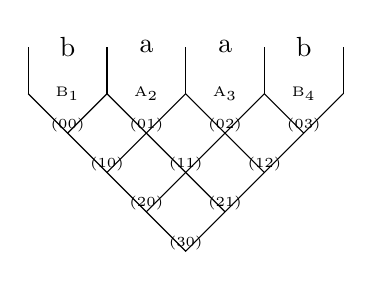
\begin{tikzpicture}[baseline]
					\newcommand{\myfontvars}[1]{
						\fontsize{4.9}{12}\selectfont{#1}
					}\newcommand{\myfontnumbering}[1]{
						\fontsize{2.5}{12}\selectfont{#1}
					}%Outer hull
					%Tip of the pyramid
					\coordinate (tip) at (2.0,-2.0);
					\foreach \i in {0,...,4} {
						\coordinate (\i) at (\i,0);
					}
					%Draw the left and right line of the pyramid pointing downwards
					\draw (0) -- (tip) -- (4);
					%Grid lines direction down-left to top-right
					\coordinate (dl1) at (0.5,-0.5);
					\coordinate (dl2) at (1.0,-1.0);
					\coordinate (dl3) at (1.5,-1.5);
					\draw (dl1) -- (1,0);
					\draw (dl2) -- (2,0);
					\draw (dl3) -- (3,0);
					%Grid lines direction down-right to top-left
					\coordinate (dr1) at (2.5,-1.5);
					\coordinate (dr2) at (3.0,-1.0);
					\coordinate (dr3) at (3.5,-0.5);
					\draw (dr1) -- (1,0);
					\draw (dr2) -- (2,0);
					\draw (dr3) -- (3,0);
					%Small lines at the top
					\coordinate (top0) at (0.0,0.0);
					\coordinate (top1) at (1.0,0.0);
					\coordinate (top2) at (2.0,0.0);
					\coordinate (top3) at (3.0,0.0);
					\coordinate (top4) at (4.0,0.0);
					\coordinate (topUpper0) at (0.0,0.6);
					\coordinate (topUpper1) at (1.0,0.6);
					\coordinate (topUpper2) at (2.0,0.6);
					\coordinate (topUpper3) at (3.0,0.6);
					\coordinate (topUpper4) at (4.0,0.6);
					\draw (top0) -- (topUpper0);
					\draw (top1) -- (topUpper1);
					\draw (top2) -- (topUpper2);
					\draw (top3) -- (topUpper3);
					\draw (top4) -- (topUpper4);
					%The string
					\coordinate (w0) at (0.5,0.6);
					\coordinate (w1) at (1.5,0.6);
					\coordinate (w2) at (2.5,0.6);
					\coordinate (w3) at (3.5,0.6);
					\node [] at (w0) {b};
					\node [] at (w1) {a};
					\node [] at (w2) {a};
					\node [] at (w3) {b};
					% Variables in the cells
					%cells00
					\coordinate (center00) at (0.5,0.0);
					\node [below=0.18cm] at (center00) {\myfontnumbering{$(00)$}};
					\node [] at (center00) {\myfontvars{B$_{1}$}};
					%cells01
					\coordinate (center01) at (1.5,0.0);
					\node [below=0.18cm] at (center01) {\myfontnumbering{$(01)$}};
					\node [] at (center01) {\myfontvars{A$_{2}$}};
					%cells02
					\coordinate (center02) at (2.5,0.0);
					\node [below=0.18cm] at (center02) {\myfontnumbering{$(02)$}};
					\node [] at (center02) {\myfontvars{A$_{3}$}};
					%cells03
					\coordinate (center03) at (3.5,0.0);
					\node [below=0.18cm] at (center03) {\myfontnumbering{$(03)$}};
					\node [] at (center03) {\myfontvars{B$_{4}$}};
					%cells10
					\coordinate (center10) at (1.0,-0.5);
					\node [below=0.18cm] at (center10) {\myfontnumbering{$(10)$}};
					%cells11
					\coordinate (center11) at (2.0,-0.5);
					\node [below=0.18cm] at (center11) {\myfontnumbering{$(11)$}};
					%cells12
					\coordinate (center12) at (3.0,-0.5);
					\node [below=0.18cm] at (center12) {\myfontnumbering{$(12)$}};
					%cells20
					\coordinate (center20) at (1.5,-1.0);
					\node [below=0.18cm] at (center20) {\myfontnumbering{$(20)$}};
					%cells21
					\coordinate (center21) at (2.5,-1.0);
					\node [below=0.18cm] at (center21) {\myfontnumbering{$(21)$}};
					%cells30
					\coordinate (center30) at (2.0,-1.5);
					\node [below=0.18cm] at (center30) {\myfontnumbering{$(30)$}};
					\end{tikzpicture}
				}	
			}
		}
	\end{minipage}
\end{figure}\\
that rules like $lhse \rightarrow CC$ or $lhse \rightarrow SC$ are added, that obviously not directly help to fill the parsing table and bloat the grammar with useless rules. More reasonably rules to add would be $lhse \rightarrow BA$, $lhse \rightarrow AA$ and $lhse \rightarrow AB$.\\
Algorithm \ref{BottomUpDiceRollVar1} takes this up: After distributing the terminals (Line \ref{var1A}) the updated parsing table (Line \ref{var1Update}) is always taken into consideration while choosing variable compounds to add (Line \ref{var1E}). I.e. for each chosen cell a $CellSet$ is calculated, that only contains reasonably variable compounds. Now only variable compounds are added that directly help to fill the parsing table.\\

\noindent
\frame{
	\begin{algorithm}[H] %or another one check
		\caption{BottomUpDiceRollVar1}
		\label{BottomUpDiceRollVar1}
		\SetAlgoLined
		\KwIn{Word $w \in \Sigma^{*}$ }
		\KwOut{Set of productions $P$}
		$P = \emptyset$;~~\tcp{$P \subseteq V \times (V^{2} \cup \Sigma)$}
		$P = Distribute(\Sigma,\ V)$;  \circled{A}\\
		$Pyramid = CYK(G,\ w)$\label{stepii}\;
		\For{$i:=1\ \textbf{to}\ i_{max}$}{
			$J = \{0,~...~,~j_{max} -1\}$;~~\tcp{$J \subseteq \mathbb{N}$}
			$CellSet = \emptyset$;~~\tcp{$CellSet \subseteq V^2$} \label{var1A}
			\While{$|J|>0$}{
				$choose\ one\ j \in J\ uniform\ randomly$\label{chooseJ}\;
				$J = J \setminus \{j\} $\;
				$CellSet = CalculateSubsetForCell(Pyramid,\ i,\ j)$;  \circled{D} \label{var1E}\\
				$P \cup Distribute(CellSet,\ V)$;  \circled{B}\\
				$Pyramid = CYK(G,\ w)$\; \label{var1Update}
				\If{$stopping\ criteria~met$~\circled{C}}{
					\Return $P$\;
				}
			}
		}
		\Return $P$\;
		\footnotetext{
			\noindent Line \ref{stepii}: Fills the i=0 row of the pyramid.
			
			\noindent Line \ref{chooseJ}: A cell is only visited only once.
		}
	\end{algorithm}
}

\pagebreak
\subsection{BottomUpDiceRollVar2}
While examining the Algorithm \ref{BottomUpDiceRollVar1} via its log files [XXX] it can be seen that already a very small number of rules in the grammar is sufficient so that the stopping criteria \circled{C} is met \textendash~the cells that indirectly decide what rules to add are mostly from row one ($i=1$) and sometimes if at all from row two ($i\leq2$).\\ 
This again leads to another idea to introduce a row dependent $threshold_i$ (Line \ref{var2threshold}) that helps that more cells with $i\geq2$ are chosen \textendash~what possibly can lead to more diverse grammars. The diversity, in context of Algorithm \ref{BottomUpDiceRollVar1}, is somewhat too restricted to the $lhse$s that have one of the terminals as its $rhse$. Most of the rules that are part of the grammar will contain one these $lhse$s. This is due to the basic idea of Algorithm \ref{BottomUpDiceRollVar1} but also due to the relatively small number of rules in the grammar. \\

\noindent
\frame{
	\begin{algorithm}[H] %or another one check
		\caption{BottomUpDiceRollVar2}
		\label{BottomUpDiceRollVar2}
		\SetAlgoLined
		\KwIn{Word $w \in \Sigma^{*}$ }
		\KwOut{Set of productions $P$}
		$P = \emptyset$;~~\tcp{$P \subseteq V \times (V^{2} \cup \Sigma)$}
		$RowSet = \emptyset$;~~\tcp{$RowSet \subseteq \{(XY,i)\ |\ X,Y \in V \wedge i \in \mathbb{N} \}$}
		$P = Distribute(\Sigma,\ V)$;  \circled{A}\\
		$Pyramid = CYK(G,\ w)$ \label{stepii}\;
		\For{$i:=1\ \textbf{to}\ i_{max}$}{
			%$choose\ j\ uniform\ randomly\ in\ [0,\ j_{max}-i]  $\;
			\For{$j:=0\ \textbf{to}\ j_{max}-i$}{
				$RowSet \cup \{(XY,i)\ |\ XY \in CalculateSubsetForCell(Pyramid,\ i,\ j) $\circled{D}$\}$\label{rowSet}\;  
			}
			\While{$threshold_i\ not\ reached $}{ \label{var2threshold}
				$choose\ one~xy\ out\ of\ (XY,\ i) \in RowSet~uniform\ randomly\ with$ $probability~depending~on~i $;\label{chooseVc} \circled{E}  \\
				$P \cup Distribute(xy,\ V) $; \circled{B}  \\
				$Pyramid = CYK(G,\ w)$\;
				\If{$stopping\ criteria~met$~\circled{C}}{
					\Return $P$\;
				}	
			}
		}
		\Return $P$\;
		\footnotetext{
			\noindent Line \ref{stepii}: Fills the i=0 row of the pyramid.
		}
	\end{algorithm}
}



\pagebreak
\subsection{SplitThenFill}

The idea here is to first distribute the terminals (Line \ref{splitThenStepii} of Algorithm \ref{SplitThenFillPrep}) and then to uniform randomly generate a predefined structure of the derivation tree (Line \ref{splitThenFillTreeStart} of Algorithm \ref{splitThenStepii} and in general Algorithm \ref{SplitThenFill}) Top-Downwards and afterwards to fill the parsing table Bottom-Upwards accordingly to this derivation tree.\\
Every time before adding a new rule the already available information regarding the other rules is used to determine if a new rule is needed to fill this node of the derivation tree (Line \ref{empty} of Algorithm \ref{SplitThenFill}).\\

\noindent
\frame{
	\begin{algorithm}[H] %or another one check
		\caption{SplitThenFillPrep}
		\label{SplitThenFillPrep}
		\SetAlgoLined
		\KwIn{Word $w \in \Sigma^{*}$}
		\KwOut{Set of productions $P$}
		$P = \emptyset$;~~\tcp{$P \subseteq V \times (V^{2} \cup \Sigma)$}
		$P = Distribute(\Sigma,\ V)$; \circled{A} \label{splitThenStepii}  \\		
		$Sol = (P_{Sol},~Cell_{i,j})$;~~\tcp{$P_{Sol} \subseteq P~\wedge~ Cell_{i,j} \in Pyramid$} \label{cell}
		$Sol = SplitThenFill(P,\ w,\ i_{max},\ 0)$\; \label{splitThenFillTreeStart}
		\Return $P_{Sol}$\;
		\footnotetext{
			\noindent Line \ref{splitThenStepii}: Fills the i=0 row of the pyramid.	
		}
	\end{algorithm}
}
\\
For this algorithm it is important to mention that while using \circled{B} (Line \ref{splitThenFillB} of Algorithm \ref{SplitThenFill}) a variable compound is added to at least one $lhse$. For every element of $Vc$ (Line \ref{splitThenFillVc} of Algorithm \ref{SplitThenFill}) there exists at least one rule $lhse \rightarrow vc$ with $vc \in Vc$.\\

\noindent
\frame{
	\begin{algorithm}[H] %or another one check
		\caption{SplitThenFill}
		\label{SplitThenFill}
		\SetAlgoLined
		\KwIn{$P_{in} \subseteq V \times (V^{2} \cup \Sigma),\ w \in \Sigma^{*},\ i,j \in \mathbb{N}$ }
		\KwOut{$(P,~Cell_{i,j})$}
		$P =  P_{in}$\;
		\If{$i=0$}{
			\Return $(P,\ Cell_{i,j})$\label{row0}\;
		}	
		$choose\ one\ m\ uniform\ randomly\ in\ [j+1,\ j+i]$\;
		$(P,\ Cell_l) = SplitThenFill(P,\ w,\ (m-j-1),\ j)$\label{left}\;
		$(P,\ Cell_r) = SplitThenFill(P,\ w,\ (j+i-m),\ m)$\label{right}\;
		$Pyramid = CYK(G,\ w)$\label{cyk}\;
		\If{$stopping\ criteria~met$~\circled{C}}{
			\Return $(P,\ Cell_{i,j})$\;
		}
		\If{$Cell_{i,j} = \emptyset$}{ \label{empty}
			$Vc = uniform\ random\ subset\ from\ \{vc\ |\ v \in Cell_l\ \wedge\ c \in Cell_r\} ~with~|Vc| \geq 1$\; \label{splitThenFillVc}
			$P \cup Distribute(Vc,\ V) $; \circled{B} \label{splitThenFillB}  \\
		}
		
		\Return $(P,\ Cell_{i,j})$\;
	\end{algorithm}
}
\pagebreak

\subsection{SplitAndFill}

It is dependent on the length of the word.\\
It is important that the terminals and the varcomps are distributed to exactly one var.
The stopping criteria will be that each cell with index i = 0 must be not empty.
Now there is a second option to fill the parse table:
\begin{enumerate}
	\item Top Down: The parse table is filled quiet unevenly. You don't have all information available. Think about adding a production for the node cell: You can add a production so that its producing cells fill the node cell, but you don't know what actually would be the best to fill in these producing cells because they themselves aren't looked at yet. This problem is kept until the last depth of the recursion, where the cells in row $i=0$ are taken into account. Only starting there you know what variables actually produce the terminals.\\
	Maybe solution: For the Top Down approach, don't assume that the terminals are already distributed over the V. Distribute the terminals over the variables in an ideal way that fits your already generated productions best.
\end{enumerate}
The problem is that we have as much productions as splits in the derivation tree exist. The productions count can be reduced via merging duplicate productions and via reducing the split count in the tree. \\
Merging productions means: If there are A --> BS and C --> BS then only one Production of these two can remain.\\

\pagebreak
\noindent
\frame{
	\begin{algorithm}[H] %or another one check
		\caption{SplitAndFillPrep}
		\label{SplitAndFillPrep}
		\SetAlgoLined
		\KwIn{Word $w \in \Sigma^{*}$}
		\KwOut{Set of productions $P$}
		$P = \emptyset$;~~\tcp{$P \subseteq V \times (V^{2} \cup \Sigma)$}
		$Sol = (P_{Sol},~v)$;~~\tcp{$P_{Sol} \subseteq P$} \label{cell}
		$Sol = SplitAndFill(P,\ w,\ i_{max},\ 0)$\;
		$Merge~productions~with~the~same~variableCompound~in~P_{Sol}$\;
		\Return $P_{Sol}$\;
		\footnotetext{
		}
	\end{algorithm}
}

\noindent
\frame{
	\begin{algorithm}[H] %or another one check
		\caption{SplitAndFill}
		\label{SplitAndFill}
		\SetAlgoLined
		\KwIn{$P_{in} \subseteq V \times (V^{2} \cup \Sigma),\ w \in \Sigma^{*},\ i,j \in \mathbb{N}$ }
		\KwOut{$(P,~v)$}
		$P = P_{in}$\;
		\If{$i=0$}{
			\Return $(P \cup (v,~ w_j),\ v_{lhse})$\;
		}
		$choose\ one\ m\ uniform\ randomly\ in\ [j+1,\ j+i]$\;
		$(P,\ v_l) = SplitAndFill(P,\ w,\ (m-j-1),\ j)$\label{left}\;
		$(P,\ v_r) = SplitAndFill(P,\ w,\ (j+i-m),\ m)$\label{right}\;	
		\If{$i=i_{max}$}{
			\Return $(P \cup (S,~v_l v_r),\ v)$\;
		}
		\Return $(P \cup (v,~v_l v_r),\ v)$\;
		\footnotetext{
		}
	\end{algorithm}
}
\\


\pagebreak
\subsection{Comparision of Algorithms} \label{ComparisonOfAlgorithms}
\noindent Write about the standard configuration used.
\begin{table}[H]
	\centering
	\begin{tabular}{ | l | c |c |c |c | }
		\hline
Algorithm 		& SR 	& SR-Producibility 	& SR-Cardinality-Rules 	& SR-Pyramid   	\\ \hline
\hline
DiceRollOnly 	& 09~\%	& 24~\% & 88~\% & 39~\%		\\ \hline
BotomUpVar1 	& 16~\% & 52~\% & 90~\% & 41~\% 	\\ \hline
BotomUpVar2 	& 19~\% & 47~\% & 93~\% & 53~\% 	\\ \hline
SplitThenFill 	& 24~\% & 40~\% & 97~\% & 67~\% 	\\ \hline
SplitAndFill 	& 11~\% & 100~\% & 69~\% & 15~\% 	\\ \hline
	\end{tabular}
	\caption{Comparison of the SRs of the algorithms. Stopping criteria root not empty.}
	\label{comparisonAlgorithms}
\end{table}
Finding of ideal parameter for each algorithm.

\begin{table}[H]
	\centering
	\begin{tabular}{ | l | c |c |c |c | }
		\hline
		Algorithm 		& SR 	& SR-Producibility 	& SR-Cardinality-Rules 	& SR-Pyramid   	\\ \hline
		\hline
		DiceRollOnly 	& 09~\%	& 23~\% & 88~\% & 38~\%		\\ \hline
		BotomUpVar1 	& 11~\% & 30~\% & 99~\% & 58~\% 	\\ \hline
		BotomUpVar2 	& 13~\% & 26~\% & 99~\% & 66~\% 	\\ \hline
		SplitThenFill 	& 24~\% & 40~\% & 97~\% & 67~\% 	\\ \hline
		SplitAndFill 	& 11~\% & 100~\% & 70~\% & 14~\% 	\\ \hline
	\end{tabular}
	\caption{Comparison of the SRs of the algorithms. Stopping criteria more than half.}
	\label{comparisonAlgorithms}
\end{table}



\begin{table}[]
	\centering
	\caption{My caption}
	\label{my-label}
	\begin{tabular}{|l|c|c|c|c|c|c|c|}
		\hline
		\multicolumn{1}{|c|}{Algorithm} & SR   & \begin{tabular}[c]{@{}c@{}}Produci-\\ bility\end{tabular} & \begin{tabular}[c]{@{}c@{}}Cardinality-\\ Rules\end{tabular} & \multicolumn{4}{c|}{Pyramid}                                                                                                                                                        \\ \cline{6-8} 
		&      &                                                           &                                                              &      & \begin{tabular}[c]{@{}c@{}}Force-\\ Right\end{tabular} & \begin{tabular}[c]{@{}c@{}}Vars-\\ PerCell\end{tabular} & \begin{tabular}[c]{@{}c@{}}VarsIn-\\ Pyramid\end{tabular} \\ \hline
		DiceRollOnly                    & 09\% &                                                           &                                                              & 67\% &                                                        &                                                         &                                                           \\ \hline
		BottomUpVar1                    &      &                                                           &                                                              &      &                                                        &                                                         &                                                           \\ \hline
		BottomUpVar2                    &      &                                                           &                                                              &      &                                                        &                                                         &                                                           \\ \hline
		SplitThenFill                   &      &                                                           &                                                              &      &                                                        &                                                         &                                                           \\ \hline
		SplitAndFill                    &      &                                                           &                                                              &      &                                                        &                                                         &                                                           \\ \hline
	\end{tabular}
\end{table}
\pagebreak